\documentclass[12pt]{article}
\setlength{\oddsidemargin}{0in}
\setlength{\evensidemargin}{0in}
\setlength{\textwidth}{6.5in}
\setlength{\parindent}{0in}
\setlength{\parskip}{\baselineskip}

\usepackage{amsmath,amsfonts,amssymb}
\usepackage{graphicx}
\usepackage{fancyhdr}
\usepackage{float}
\pagestyle{fancy}


\begin{document}

\lhead{{\bf CSCI 3104: Algorithms \\ Problem Set 7 (110 total points)} }
\rhead{{\bf Instructor\ Buxton\\ Summer 2019, CU-Boulder}}
\renewcommand{\headrulewidth}{0.4pt}

\vspace{-3mm}
\begin{enumerate}
	% HARD PROBLEM
	\item (30 points) Grog gives you the following unweighted graph and asks you to construct a weight function $w$ on the edges, using positive integer weights only, such that the following conditions are true regarding minimum spanning trees (MST) and single-source shortest path trees (SSSP):
	\begin{itemize}
	\itemsep-0.1pt
	\item The MST is distinct from any of the seven SSSP trees.
	\item The order in which Jarn\'ik/Prim's algorithm adds the safe edges is different from the order in which Kruskal's algorithm adds them.
	\end{itemize}
	Justify your solution by (i) giving the edges weights, (ii) showing the corresponding MST and all the SSSP trees, and (iii) giving the order in which edges are added by each of the two algorithms.

    % ----- FIGURE 1 : unweighted_graph.png -----
    \begin{figure}[h!]
    \begin{center}
    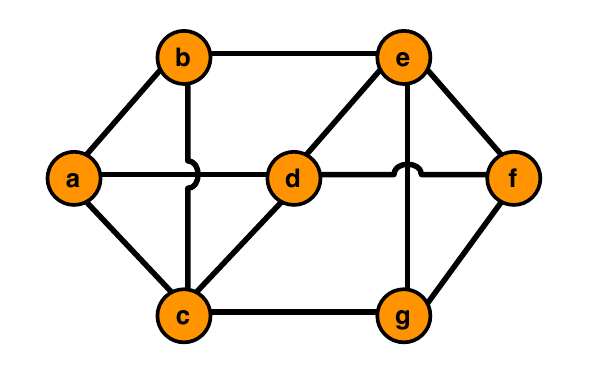
\includegraphics[scale=0.7]{unweighted_graph.png} 
    \end{center}
    \end{figure}
    % ----------

    \pagebreak

	
	% CURRENCY ARBITRAGE
	\item (25 points) Harry and Shadow think they have come up with a way to get rich by exploiting the ore market. Their idea is to exploit exchange rates in order to transform one unit of gold into more than one unit of gold, through a sequence of exchanges. For instance, suppose 1 unit of gold buys 0.82 silver units, 1 silver unit buys 129.7 ethereum units, 1 ethereum unit buys 12 doge units, and finally 1 doge unit buys 0.0008 gold units. By converting their loot, Harry and Shadow think they could start with 1 gold unit and buy $0.82 \times 129.7 \times 12 \times 0.0008 \approx 1.02$ gold units, thereby making a 2\% profit! The problem is that those dwarves at Rocky  Mountain  Bank  charge a transaction cost for each exchange.
	
	Suppose that Harry and Shadow start with knowledge of $n$ ores $c_{1},c_{2},\dots,c_{n}$ and an $n\times n$ table $R$ of exchange rates, such that one unit of ore $c_{i}$ buys $R[i,j]$ units of ore $c_{j}$. A traditional \textit{arbitrage opportunity} is thus a cycle in the induced graph such that the product of the edge weights is greater than unity. That is, a sequence of ores $\langle c_{i_{1}} , c_{i_{2}}, \dots, c_{i_{k}}\rangle$ such that $R[i_{1}, i_{2}] \times R[i_{2}, i_{3}] \times \cdots \times R[i_{k-1}, i_{k}] \times R[i_{k}, i_{1}] > 1$. Each transaction, however, must pay Rocky  Mountain  Bank a fraction $\alpha$ of the total transaction value, e.g., $\alpha=0.01$ for a 1\% rate.

	\begin{enumerate}
	\item When given $R$ and $\alpha$, give an efficient algorithm that can determine if an arbitrage opportunity exists. Analyze the running time of your algorithm.
	
	Thormund's hint:\ It is possible to solve this problem in $O(n^{3})$. 
	\item For an arbitrary $R$, explain how varying $\alpha$ changes the set of arbitrage opportunities that exist and that your algorithm might identify.
	\end{enumerate}
    
    \pagebreak
	
	% PROGRAMMING PROBLEM
	\item (55 points) Bidirectional breadth-first search is a variant of standard BFS for finding a shortest path between two vertices $s,t \in V(G)$. The idea is to run \emph{two} breadth-first searches simultaneously, one starting from $s$ and one starting from $t$, and stop when they ``meet in the middle'' (that is, whenever a vertex is encountered by both searches). ``Simultaneously'' here doesn't assume you have multiple processors at your disposal; it's enough to alternate iterations of the searches: one iteration of the loop for the BFS that started at $s$ and one iteration of the loop for the BFS that started at $t$.
	
	As we'll see, although the worst-case running time of BFS and Bidirectional BFS are asymptotically the same, in practice Bidirectional BFS often performs significantly better.
	
	Throughout this problem, all graphs are unweighted, undirected, simple graphs.
	
	\begin{enumerate}
	
	\item Implement from scratch a function \texttt{BFS(G,s,t)} that performs an ordinary BFS in the (unweighted, directed) graph $G$ to find a shortest path from $s$ to $t$. Assume the graph is given as an adjacency list; for the list of neighbors of each vertex, you may use any data structure you like (including those provided in standard language libraries). Have your function return a pair $(d,k)$, where $d$ is the distance from $s$ to $t$ (-1 if there is no $s$ to $t$ path), and $k$ is the number of nodes popped off the queue during the entire run of the algorithm.
	
	\item Implement from scratch a function  \texttt{BidirectionalBFS(G,s,t)} that takes in an unweighted, directed graph $G$, and two of its vertices $s,t$, and performs a bidirectional BFS. As with the previous function, this function should return a pair $(d,k)$ where $d$ is the distance from $s$ to $t$ (-1 if there is no path from $s$ to $t$) and $k$ is the number of vertices popped off of both queues during the entire run of the algorithm.
	
	\item For each of the following families of graphs $G_n$, write code to execute $\texttt{BFS}$ and $\texttt{BidirectionalBFS}$ on these graphs, and produce the following output: 
	\begin{itemize}
	\item In text, the pairs $(n,d_1,k_1,d_2,k_2)$ where $n$ is the index of the graph, $(d_1,k_1)$ is the output of $\texttt{BFS}$ and $(d_2, k_2)$ is the output of $\texttt{BidirectionalBFS}$. 
	\item a plot with $n$ on the $x$-axis, $k$ on the $y$-axis, and with two line charts, one for the values of $k_1$ and one for the values of $k_2$:
	\end{itemize}
	
	\begin{enumerate}
	\item Grids. $G_n$ is an $n \times n$ grid, where each vertex is connected to its neighbors in the four cardinal directions (N,S,E,W). Vertices on the boundary of the grid will only have 3 neighbors, and corners will only have 2 neighbors. Let $s_n$ be the midpoint of one edge of the grid, and $t_n$ the midpoint of the opposite edge. For example, for $n=3$ we have:
    \begin{figure}[H]
    \begin{center}
    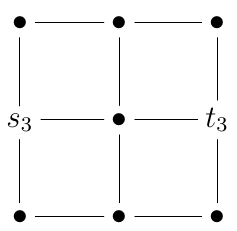
\includegraphics[scale=0.9]{grid.png} 
    \end{center}
    \end{figure}

	(When $n$ is even $s_n$ and $t_n$ can be either ``midpoint,'' since there are two.)
	
	Produce output for $n=3,4,5,\dotsc,20$.
	
	\item Trees. $G_n$ is a complete binary tree of depth $n$. $s_n$ is the root and $t_n$ is any leaf. Produce output for $n=3,4,5,\dotsc,15$. For example, for $n=3$ we have:
    \begin{figure}[H]
    \begin{center}
    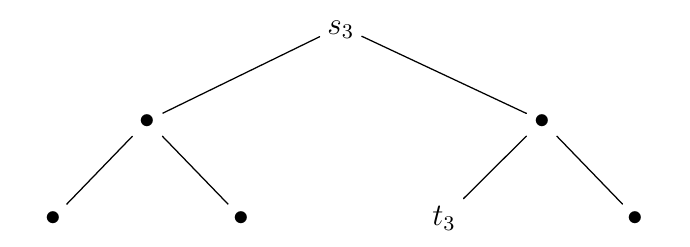
\includegraphics[scale=0.6]{tree.png} 
    \end{center}
    \end{figure}
		
	\item Random graphs. $G_n$ is a graph on $n$ vertices constructed as follows. For each pair of of vertices $(i,j)$, get a random boolean value; if it is \texttt{true}, include the edge $(i,j)$, otherwise do not. Let $s_n$ be vertex 1 and $t_n$ be vertex 2 (food for thought: why does it not matter, on average, which vertices we take $s,t$ to be?) For each $n$, produce 50 such random graphs and report just the average values of $(d_1,k_1,d_2,k_2)$ over those 50 trials. Produce this output for $n=3,4,5,\dotsc,20$.
	\end{enumerate}
	\end{enumerate}
	
\end{enumerate}
\end{document}


